\documentclass[
 preprint,
 preprintnumbers,
 amsmath,amssymb,
 aps,
 pre,
 longbibliography,
 superscriptaddress,
 10pt, twocolumn
]{revtex4-1}

\usepackage{graphicx}% Include figure files
\graphicspath{{./figures/}} % path to figures
\usepackage{dcolumn}% Align table columns on decimal point
\usepackage{bm}% bold math
\usepackage{hyperref}% add hypertext capabilities
\usepackage{physics} % package for physics symbols

\begin{document}
% define commands
\newcommand{\eqnname}{Eqn.}
\newcommand{\secname}{Sec.}


\title{Rectification of energy and motion in active gyroscopic networks}


\author{Zhenghan Liao}
\affiliation{Department of Chemistry, University of Chicago, Chicago, IL, 60637, USA}
\author{William Irvine}
\affiliation{James Franck Institute, Enrico Fermi Institute and Department of Physics, University of Chicago, Chicago, IL, 60637, USA}
\author{Suriyanarayanan Vaikuntanathan}
\affiliation{James Franck Institute and Department of Chemistry, University of Chicago, Chicago, IL, 60637, USA}


\begin{abstract}
[Will be revised in the end] We study a model that combines gyroscopic networks and active matter. From numerical calculations, theory, and simulations, we show that autonomous heat flows are generated at the nonequilibrium steady state. Distinct from conventional heat flows that are driven by temperature difference at the boundaries, this heat flow is an emergent collective behavior.
We then focus on understanding three issues: the mechanism of this nonzero heat flow, the connection between the flow in active system and that in the well-studied isolated system, and the relationship between the network geometry and the flow pattern.
Understanding the last issue in turn enables us to control the flow pattern by the design of the network geometry.
\end{abstract}

\maketitle

\section{Introduction} \label{sec:intro}

%Active matter studies systems where each individual component consumes energy and is driven out of equilibrium.
%This field was largely inspired by natural phenomena like bird flocking and fish schooling, where these active components act together and generate rich collective motions.
%Since then, the field has been fast-growing, expanding its interest to a broad range of systems.
%Recently, a few efforts combined ingredients from active matter and ideas from topological metamaterials, another rich field, and resulted in interesting phenomena, including topological sound in active liquid (Anton, Shankar), actuation of zero modes \cite{Woodhouse2018AutonomousActuation}, and active topolectrical circuits (Kotwal).

%Along similar lines, we study a combination of active matter and gyro metamaterials (Nash).
%We show that, at its nonequilibrium steady state, the system generates energy flux between sites.
%This energy transport is distinct from the conventional ones, since conventional energy flows are driven by temperature differences, whereas in our system, baths on all our sites are identical.
%In other words, our system can rectify energy in the absence of apparent asymmetries or biases.
%Indeed, usually energy are transported between terminals that differ in some aspects, either in temperatures, or in electrical potentials as in thermoelectric effect.
%In some more recent studies, unconventional energy transport can happen in thermal Hall effect as a transverse flow, or in thermal ratcheting using time-periodic protocols \cite{Li2008RatchetingHeat,Ren2010EmergenceControl,Ren2012GeometricHeat}, or between non-Gaussian baths with different higher-order moments \cite{Kanazawa2013HeatConduction}.
%However, rarely do people study energy flux in a system where all terminals are identical, because the flux in this case should be zero. One rare case of violation is heat radiation in a special equilibrium system with nonreciprocal magneto-optical nanoparticles \cite{Zhu2016PersistentDirectional}.

%Our system is not only able to achieve rectification of energies, but also able to control the rectification using network geometries.
%We analytically and numerically demonstrate these results for a wide variety of network geometries thus establishing the generality of our results. In particular, we construct an intuitive diagrammatic approach for computing the energy flux that shows how our results can readily applied to tailor flows in arbitrarily complex networks.
%Taken together, our results establish a new set of design principles for rectification in many body systems. Our design principles, unlike many existing prescriptions, exploit inherent asymmetries in the geometry and interactions of the material to achieve rectification.

One of the longstanding problems in non-equilibrium statistical mechanics concerns uncovering principles for the rectification of energy and motion in many body microscopic systems~\cite{seifert2012stochastic,coskun2012great}. The Feynman Ratchet and pawl model, and its associated generalizations, have elucidated how a combination of spatial asymmetry and non-equilibrium forcing can lead to rectification of current and work generation in simple low dimensional model systems~\cite{jarzynski1999feynman}. Brownian ratchet models have also provided a framework to understand how molecular motors and biophysical polymers like actin transmit and exert forces~\cite{mogilner1996cell}. New theoretical results, such as the no pumping theorems have provided a minimal set of constraints for changing the kinetic rates in a ratchet model to ensure rectification~\cite{Chernyak2008,Rahav2008,Sinitsyn2007}. Despite these advances, we still have very few design principles to engineer rectification in many body systems~\cite{seifert2012stochastic}. This is a current and relevant problem of interest, especially given the recent progress made in the in study of so called active matter systems where energy injection at the microscopic level results in larger scale reorganization ~\cite{marchetti2013hydrodynamics,souslov2017topological,Shankar2017}.In this paper, we attempt to address a limited version of the problem and show energy and motion can be rectified in a class of model systems composed of chiral meta-materials interacting with an active bath.

Designs of mechanical metamaterials have achieved unconventional mechanical properties or functions in a wide range of systems \cite{Bertoldi2017FlexibleMechanical}. Examples include negative Poisson ratios in auxetic metamaterials \cite{Lakes2017NegativePoissonSRatio,Ren2018AuxeticMetamaterials}, topological zero modes in isostatic lattices \cite{Kane2013TopologicalBoundary,Lubensky2015PhononsElasticity,Paulose2015SelectiveBuckling}, unidirectional edge modes in topological gyroscopic metamaterials \cite{Nash2015TopologicalMechanics,Wang2015TopologicalPhononic,Mitchell2018AmorphousTopological}, and the allosteric effect in mechanical networks \cite{Rocks2017DesigningAllosteryinspired,Yan2017ArchitectureCoevolution,Flechsig2017DesignElastic}. In particular, studies of gyroscopic chiral metamaterials have shown how peculiar topological edge modes, where the energy circulates along the network boundary unidirectionally, can be supported in classical systems\cite{Nash2015TopologicalMechanics}. These topological chiral edge modes can be explained in terms of a violation of time reversal symmetry in the microscopic equations of motion of the interacting gyroscopes~\cite{Nash2015TopologicalMechanics,Mitchell2018AmorphousTopological}. Importantly, the violation of time reversal symmetry is controlled by an interplay between the spin of the gyroscopes and the geometry of the lattice.

%In contrast to the increasing studies on mechanical properties, one less explored topic is the effect of thermal fluctuations{\bf rewrite sentence, awkward construction}. This effect is usually irrelevant, because the energy scale of the metamaterials is much larger than that of thermal fluctuations. However, fluctuations are inevitable if the system is made in micro-scale \cite{Blees2015GrapheneKirigami}.
% Indeed, some recent works have found an interesting interplay between thermal \cite{Rocklin2018FoldingMechanisms,Pedro2018TopologicalProtection} or nonequilibium \cite{Woodhouse2018AutonomousActuation} fluctuations and the zero mode, which show promises in studying the effect of fluctuations.

 In this paper we show how notions of time reversal symmetry violation in chiral topological metamaterials can be combined with violations of the fluctuation dissipation relation by \textit{active} particles to rectify energy and mass flows. The active bath we use is the active Ornstein-Uhlenbeck particle (AOUP) model \cite{Fodor2016HowFar}, which consists of a constant friction and an Ornstein-Uhlenbeck (OU) noise. The AOUP model has experienced a growing interest in recent years, because of its theoretical simplicity and its ability to capture many nonequilibrium and active matter phenomena.
For instance, it has been experimentally found that, colloids in a bacteria bath can be well-modeled by the AOUP model \cite{Wu2000ParticleDiffusion}; this finding helped realized previously proposed thermal ratchet models \cite{Magnasco1993ForcedThermal} in experiments with bacterial baths. \cite{Koumakis2013TargetedDelivery}

 Our central result shows how a combination of time reversal symmetry violations due to chirality and interactions in a model system, and time reversal symmetry violations implicit in the fluctuations of the bath that the model system is in contact with, can help support rectification. In particular, we find that our combined system can support a directed flux of energy across the network. Unlike conventional energy flows, our energy flow is not supported by a temperature gradient. Moreover, the \textit{active gyroscopic} network can in fact pump energy through an otherwise isolated elastic object. We also show that the microscopic mechanisms responsible for this energy flow can also potentially allow the \textit{active gyroscopic} network to swim in and exert forces on a viscous fluid. We analytically and numerically demonstrate these results for a wide variety of network geometries thus establishing the generality of our results. In particular, we construct an intuitive diagrammatic approach for computing the energy flux (and consequently the swim speed) that shows how our results can readily applied to tailor flows in arbitrarily complex networks.

Taken together, our results establish a new set of design principles for rectification of energy, motion and forces in chiral many body systems. Our design principles, unlike many existing prescriptions, exploit inherent asymmetries in the geometry and interactions of the material to achieve rectification.


The remainder of this paper is organized as follows:
In \secname~\ref{sec:model}-\ref{sec:flux}, we introduce our model active chiral system, and provide a microscopic definition for the energy flux.
In \secname~\ref{sec:linear_response}-\ref{sec:path} we analytically identify the ingredients for rectification of energy fluxes and construct a diagrammatic approach that reveals the relationship between energy flux and network geometries.
Finally in \secname~\ref{sec:swimmer} we show how the rectified energy flows created by our system can pump energy through a material. We also show how the microscopic fluctuations that accompany a non-zero energy flux can be rectified by a viscous fluid at low Reynolds numbers. Such rectification can either allow our model systems to swim or pump fluid when their centre of mass is held fixed.
%Finally, in \secname~\ref{sec:conclusion} we


\section{Model} \label{sec:model}

\begin{figure}[ht]
	\centering
	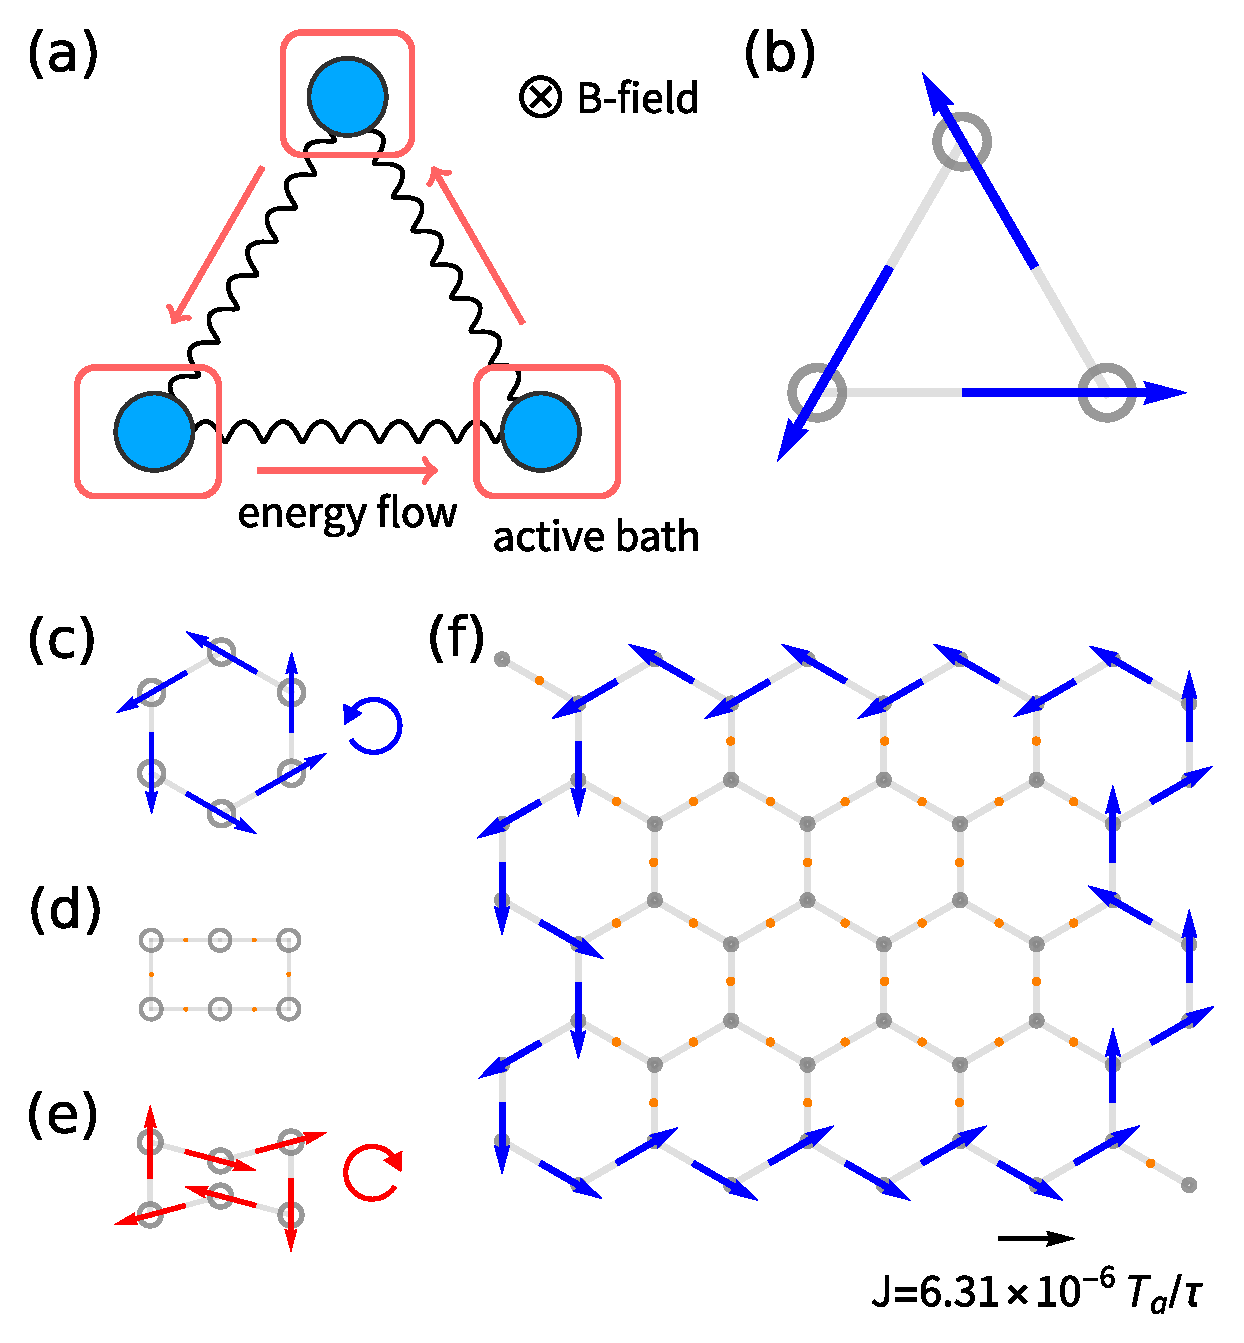
\includegraphics[width=0.45\textwidth]{1_model_and_result.pdf}
    \caption{The model and the heat flux in polygonal and more complex networks. All parameters are set to $1$.
    (a) Schematic of the model, a spring-mass network with Lorentz force and active bath on each mass.
    (b-f) Heat flux results from numerical calculations. Gray circles and lines represent the network geometry. Arrows represent the direction and magnitude of the heat flux. Fluxes are colored blue if it is counter-clockwise (CCW), red if clockwise (CW), and orange otherwise. For complex networks, fluxes smaller than $1/10$ of the scale bar are not shown for clarity.
    (b) Triangle network has CCW heat flux, $\expval{J}=1.61\times 10^{-3} T_a/\tau$.
    (c-e) In hexagon networks, the flux direction changes with the geometry. Flux magnitude in both (c),(e) is $6.26\times 10^{-6} T_a/\tau$.
    (f) The flux pattern in the honeycomb network shows localization on the boundary and CCW direction.
    }
    \label{fig:model_and_result}
\end{figure}

Our model chiral system is a spring-mass network with Lorentz-like force and active bath \cite{Fodor2016HowFar} on each site (\figurename~\ref{fig:model_and_result}a).
The equation of motion reads
\begin{equation} \label{eqn:GLE_single}
    m\dot{\bm{v}}_i = -k_g \bm{z}_i + \sum_j\bm{F}_{ji} + \bm{v}_i\times\bm{B} - \gamma\bm{v}_i + \bm{\eta}_i ,
\end{equation}
where $z_i \equiv \begin{pmatrix} x_i & y_i \end{pmatrix}^T$ is the displacement of particle $i$ from its mechanical equilibrium position.

The first three terms on the right-hand side describe a spring-mass network with Lorentz force.
The first term is the on-site restoring force.
The second term is the spring force from the bonded neighbors $j$'s,
$F_{ji} = k (e_{ij}^T z_i + e_{ji}^T z_j) (-e_{ij})$.
Here the force is linearized by assuming the natural length of springs are much larger than the scale of particles' displacement, and $e_{ij}$ is the unit vector from the equilibrium position of $i$ to that of $j$.
The third term $\bm{v}_i\times\bm{B}$ is the Lorentz-like force (the electric charge is absorbed in $\bm{B}$), and we set $\bm{B} = -B\mathbf{\hat{z}}$.
The construction of our model system is motivated by the recently constructed topological gyroscopic metamaterials \cite{Nash2015TopologicalMechanics}. Indeed, in the linearized regime, the equations of our model system are equivalent to the equations of motion of the gyroscopic metamaterials~\cite{Lee2018TopologicalDynamics}.

%We used Lorentz force instead of gyroscopes because the former is more convenient {\bf may need a better explanation}.

The last two terms describe the active bath, which consists of friction $-\gamma v_i$ and an Ornstein-Uhlenbeck (OU) colored noise $\eta_i$~\cite{Fodor2016HowFar}.
The colored noise has finite correlation time $\tau$ and strength $T_a$ ($T_a$ has the unit of energy)
\begin{equation} \label{eqn:noise_correlation}
    \expval{\eta_i(t)\eta_{j}^T(t')} = I\delta_{i,j}\frac{\gamma T_a}{\tau} e^{-\frac{|t-t'|}{\tau}} ,
\end{equation}
where $I$ is the identity matrix with appropriate dimensions.
The time evolution of the OU noise can be described according to the following equation~\cite{Hanggi1994ColoredNoisea},
\begin{equation} \label{eqn:noise_eom}
    \tau \dot{\eta}_i = -\eta_i + \sqrt{2\gamma T_a}\xi_i ,
\end{equation}
where $\xi_i$ is the standard Gaussian white noise.
The friction $-\gamma v_i$ and OU noise $\eta_i$ break fluctuation-dissipation relation, thus driving the system out of equilibrium~\cite{Fodor2016HowFar}.
The active bath reduces to the familiar Langevin bath in the $\tau \rightarrow 0$ limit.


\section{Energy flux definition and results} \label{sec:flux}
The observable we mainly focus on is the time-averaged energy flux between particles at steady state. For a system with pairwise interactions and on-site potentials, the energy flux $\expval{J_{ij}}$ from particle $i$ to $j$ reads
\begin{equation} \label{eqn:flux_def}
    \expval{J_{ij}} = \expval{\frac{1}{2} (\mathbf{v}_j \cdot \mathbf{F}_{ij} - \mathbf{v}_i \cdot \mathbf{F}_{ji})}
    = \expval{\mathbf{v}_j \cdot \mathbf{F}_{ij}}.
\end{equation}
To arrive at this formula, first we define the energy of a particle as the sum of its kinetic energy, on-site potential energy, and one half of the bond energies \cite{Lepri2003ThermalConduction}. Then we write down the energy balance relations using ideas from stochastic thermodynamics~\cite{Sekimoto1998LangevinEquation}. Finally we identify the energy exchanged due to particle-particle interactions as the energy flux $\expval{J_{ij}}$. A detailed derivation is provided in the supplemental material.
We note that the energy flux can simply be interpreted as the rate at which work is done on particle $j$ by particle $i$.
Since this microscopic work is due to particles' stochastic motions, rather than due to an external control, the energy flux can also be interpreted as a heat flux \cite{Sekimoto1998LangevinEquation,Lepri2003ThermalConduction}. The energy fluxes are identitically equal to zero for a system at equilibrium.

For our linearized systems, starting \eqnname~\eqref{eqn:GLE_single}, \eqref{eqn:noise_eom}, the energy fluxes can be readily computed numerically \cite{Gardiner2009ItoCalculus,Ceriotti2010ColoredNoiseThermostats}, given the equation of motion  (Supplemental Material).
A collection of numerical results are shown in \figurename~\ref{fig:model_and_result}. We see nonzero energy rectification or energy fluxes can be sustained in our chiral active system (\figurename~\ref{fig:model_and_result}b), and the flux direction or pattern changes with the network geometry (\figurename~\ref{fig:model_and_result}c-f). Using a linear response theory, we now obtain analytical expressions for the energy flux. These expressions reveal how a combination of geometry, chirality, and non-equilibrium activity in the bath, are responsible for sustaining energy fluxes.

% Numerical calculations of $\expval{J}$ are performed using Mathematica \cite{WolframResearch2018MathematicaVersion}



\section{Linear response theory for energy flux} \label{sec:linear_response}
%In this section, we use a linear response theory to derive formulae for the energy flux \eqnname~\eqref{eqn:flux_integral} and \eqref{eqn:flux_residue}. These two equations contain all information we need for the energy flux, however, this information is not apparent because the equations are compact.
%In the next two sections, we try to reveal the meaning of these two equations.
%\secname~\ref{sec:fourier} analyzes a generalization of \eqnname~\eqref{eqn:flux_integral}, and explains the ingredients for nonzero energy rectifications.
%\secname~\ref{sec:path} expands \eqnname~\eqref{eqn:flux_residue} as a path summation, and explains how the flux depends on the network geometry.

%define the Fourier transform (FT) of a variable $f$ over a time period $t$ as $\tilde{f}(\omega) = \frac{1}{t} \int_0^t dt'\ f(t')e^{-i\omega t'}$, and represent the displacement of all particles by a column vector $z=\sum_i \ket{i}\otimes z_i$, with $\ket{i}$ denoting the 2D subspace of $i$,
%then the FT of the equation of motion \eqnname~\eqref{eqn:GLE_single} becomes
We begin by writing the equations of motion, \eqnname~\eqref{eqn:GLE_single}, in frequency space,
\begin{gather} \label{eqn:response}
    \tilde{z}(\omega) = G^+(\omega) \tilde{\eta}(\omega), \\
    G^{+}(\omega) \equiv [K + i\omega(\gamma I + BA) - m\omega^2I]^{-1},
\end{gather}
where we have represented the displacement of all particles by a column vector $z=\sum_i \ket{i}\otimes z_i$, with $\ket{i}$ denoting the 2D subspace of $i$, $\tilde{z}(\omega)$ denotes the Fourier transform of $z$, $\tilde{\eta}(\omega)$ is the Fourier transform of the OU noise, $G^+$ is a response matrix, matrix $K$ encodes all on-site and spring forces $F$ according to $F=-Kz$, and $A$ is an antisymmetric matrix $A=\sum_i \ket{i}\bra{i}\otimes \mqty(0 & 1 \\ -1 & 0)$. This equation describes how the displacement $z$ responses to the noise $\tilde{\eta}$.

Following the procedure in \cite{Kundu2011LargeDeviations}, the flux defined in \eqnname~\eqref{eqn:flux_def} can be expressed using $G^+$ as a spectral integral (Supplemental Material)
\begin{equation} \label{eqn:flux_integral}
    \expval{J} = \int_{-\infty}^\infty \dd{\omega} \frac{1}{1+\omega^2\tau^2} [-\frac{T_a k}{2\pi} \Re \tr G^+(\omega)A^{as}] ,
\end{equation}
where $A^{as}$ is an antisymmetric matrix
$A^{as} = -\ket{i}\bra{j} \otimes e_{ij}e_{ji}^T + \ket{j}\bra{i} \otimes e_{ji}e_{ij}^T$.
The response function $G^+(\omega)$ has no pole in the lower-half complex plane, but the colored noise introduces one pole at $\omega = -i/\tau$. Using the residue theorem we get a compact expression for the energy flux in terms of the geometry of the lattice, chirality, and statistics of the OU noise (Supplemental Material)
\begin{equation} \label{eqn:flux_residue}
    \frac{\expval{J}}{T_a/\tau} = -\frac{k}{2} \tr G^+(-\frac{i}{\tau})A^{as} .
\end{equation}
\eqnname~\eqref{eqn:flux_integral} and \eqref{eqn:flux_residue} will serve as our starting point to understand the energy flux. While they contain all the information required to compute energy fluxes, they have limited utility as design principles. Indeed, as written down, they require that the flux be recomputed de novo for each new network geometry and non-equilibrium bath activity. In the next sections, we show that it is possible to expand \eqnname~\eqref{eqn:flux_integral} and \eqref{eqn:flux_residue} in forms that reveals desgin principles for controlling energy fluxes.

Before moving on, we note that the energy fluxes satisfy Kirchoff's law, $\sum_i \expval{J_{ij}} = 0$, i.e. on average there is no energy exchange between particles and the active bath. This can be shown by calculating the average heat exchange between particle $i$ and the active bath $\expval{\eta_i^T v_i - \gamma v_i^T v_i}$, which results in zero.
This Kirchoff's law puts a strong constraint on possible flux patterns among particles, and some corollaries immediately follow, such as networks with no cycles cannot have nonzero flux, and fluxes of all bonds in a polygon network (as in \figurename~\ref{fig:model_and_result}b-e) are equal.


\section{Ingredients for energy rectification and their roles} \label{sec:fourier}

\begin{figure}[ht]
	\centering
	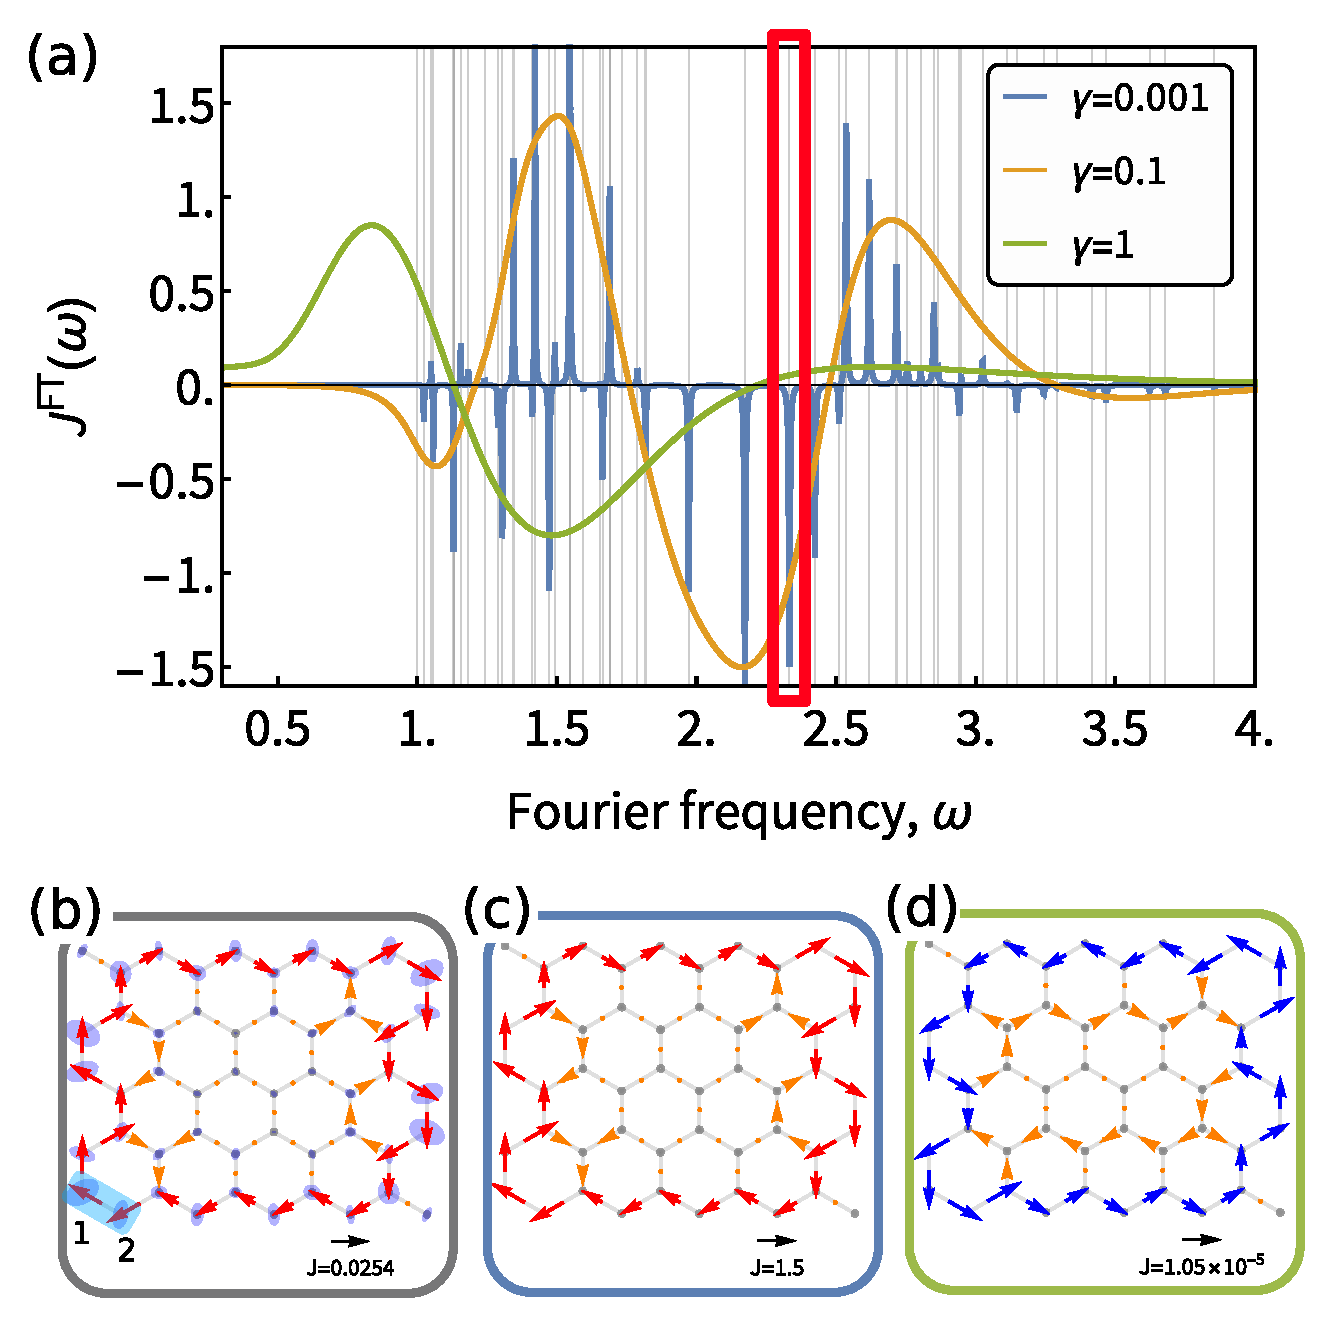
\includegraphics[width=0.45\textwidth]{2_Fourier_modes.pdf}
    \caption{The Fourier modes in the honeycomb network have nonzero fluxes, which at small $\gamma$'s originates from the chiral eigenmodes. For a better comparison between the Fourier mode and the eigenmodes studied in \cite{Nash2015TopologicalMechanics}, we use $1$st order dynamics (by setting $m=0$). All other parameters are set to $1$.
    (a) Flux $J^{FT}(\omega)$ from particle $1$ to $2$ (highlighted in (b)) as a function of Fourier frequency $\omega$ for $\gamma=0.001,0.1,1$. For plotting purposes, $J^{FT}(\omega)$ for $\gamma=0.1,1$ are scaled up by $50,5000$, respectively. Positive (negative) $J^{FT}(\omega)$ corresponds to CCW (CW) flux. Gray vertical lines mark the frequency of eigenmodes.
    (b-d) Comparison of the eigenmode and Fourier modes at frequency $2.33$.
    (b) The eigenmode is localized on the boundary. Blue disks represent the orbit of particles.
    (c) The Fourier mode at small $\gamma$'s ($\gamma=0.001$) resembles the eigenmode.
    (e) The Fourier mode at larger $\gamma$'s ($\gamma=1$) is dissimilar to the eigenmode.
    }
    \label{fig:Fourier_modes}
\end{figure}

Compared with an ordinary thermal spring-mass network which supports no energy fluxes in its equilibrium steady state, the extra components in our model are the Lorentz force and the correlation in the noise.
This section shows that these two components, in combination with network geometry provide the minimal ingredients required to ensure sustained fluxes of energy in our model.

For easier identification of the roles and later generalizations, we rewrite the integral \eqnname~\eqref{eqn:flux_integral} as $\expval{J} = \int_{-\infty}^\infty \dd{\omega} h(\omega) J^{FT}(\omega)$, with $J^{FT}(\omega) \equiv -(T_a k/2\pi) \Re \tr G^+(\omega)A^{as}$ and $h(\omega)=1/(1+\omega^2\tau^2)$. Here, we note that $J^{FT}(\omega)$ is proportional to the the energy flux at Fourier frequency $\omega$ in an isolated damped variant of our network. The function $h(\omega)$ is the the noise spectrum (apart from a prefactor of $T_a$), $\expval{\tilde{\eta}(\omega)\tilde{\eta}^*(\omega)} = 2\gamma T_a h(\omega) / t$.

To generate a nonzero flux, or equivalently make the integral nonzero, we need two requirements.
Firstly, $J^{FT}(\omega)$ should not be zero everywhere.
%This is indeed the case from numerical calculations of $J^{FT}(\omega)$ %\figurename~\ref{fig:Fourier_modes}a.
In small $\gamma$ regime, a prescription for realizing $J^{FT}(\omega) \neq 0$ can be obtained by exploiting the connection between the eigenmodes of the isolated variants of our system and the eigenmodes of topological gyroscopic metamaterials~\cite{Nash2015TopologicalMechanics}. Specifically, in the small damping region, the resonant frequencies of the damped and eigen-frequencies of the undamped system are very close. As discussed previously, the dynamics of the undamped system map on to the dynamics of topological gyroscopic mematerials \textendash these have been shown to support chiral eigenmodes~\cite{Nash2015TopologicalMechanics} (\figurename~\ref{fig:Fourier_modes}b,c). The chiral eigenmodes can support a non-zero energy flux. {\bf needs more work}

At larger $\gamma$'s, the Fourier modes of our damped isolated system are no longer close to the chiral eigenmodes of gyroscopic metamaterials (\figurename~\ref{fig:Fourier_modes}b and d), but a connection between eigenmodes and energy fluxes can still be built (Supplemental Material).
{\bf needs more transitions}
Taken together, $J^{FT}(\omega) \neq 0$ is due to the nonreciprocity induced by the Lorentz force and lattice geometry. If $B=0$, the response $G^+$ is symmetric or reciprocal, and since $A^{as}$ is antisymmetric, the trace $\tr G^+(\omega) A^{as}=0$ at all $\omega$'s. Nonzero $B$ and appropriate lattice geometry breaks the reciprocity of $G^+$, thus generating a nonzero energy flux.

Nonzero $J^{FT}(\omega)$ alone does not ensure a nonzero total flux, we further need that $h(\omega)$ should not be constant.
If $h(\omega)$ is constant, it corresponds to a white noise, and the system would be in equilibrium according to the Bohr-van Leeuwen theorem \cite{Pradhan2010NonexistenceClassical}. %In this case, the integral is always zero regardless of the value of $J^{FT}(\omega)$, because the response function $G^+(\omega)$ has no pole in the lower-half plane due to causality, consequently the flux as a contour integral vanishes.
%The conclusion of vanishing flux under white noise can also be obtained from the Bohr-van Leeuwen theorem \cite{Pradhan2010NonexistenceClassical}.

The $h(\omega)$ for the fluctuation dissipation violating OU noise, $h(\omega)=1/(1+\omega^2\tau^2)$, provides more weightage to fluxes at smaller values of $\omega$. The resulting average flux can hence potentially be non-zero. We note that other forms of colored noise could have also served the same purpose. %We chose to work with the OU noise since i
%The requirement of non constant noise spectrum indicates a nonequipartition role of the active bath \cite{Lee2017FluctuationSpectra}.
%In fact the OU noise is just one choice of the non-white noise, and any nonconstant noise spectrum $h(\omega)$ is likely to shift the integral away from zero.
%However, $h(\omega)=1/(1+\omega^2\tau^2)$ is arguably the simplest nontrivial noise.
%Because it only has one pole in the lower-half complex plane, which makes the evaluation of the integral as simple as evaluating the integrand at only one point; in addition, $\tr G^+(\omega)A^{as}$ at this pole $\omega=-i/\tau$ is real, so one can skip the evaluation of the $\Re$ part in $J^{FT}(\omega)$. As a result, the flux as an integral \eqnname~\eqref{eqn:flux_integral} can be integrated to get formula \eqnname~\eqref{eqn:flux_residue}.

In summary, we see that the main ingredients for energy rectification are the $B$-field, geometry of the lattice, and a colored noise.
The role of the $B$-field and lattice geometry is to induce chiral Fourier modes via breaking the reciprocity of response. The role of the colored noise is to excite these modes in a weighted manner.


\section{Relationship between flux and network geometry} \label{sec:path}
\begin{figure}[ht]
	\centering
	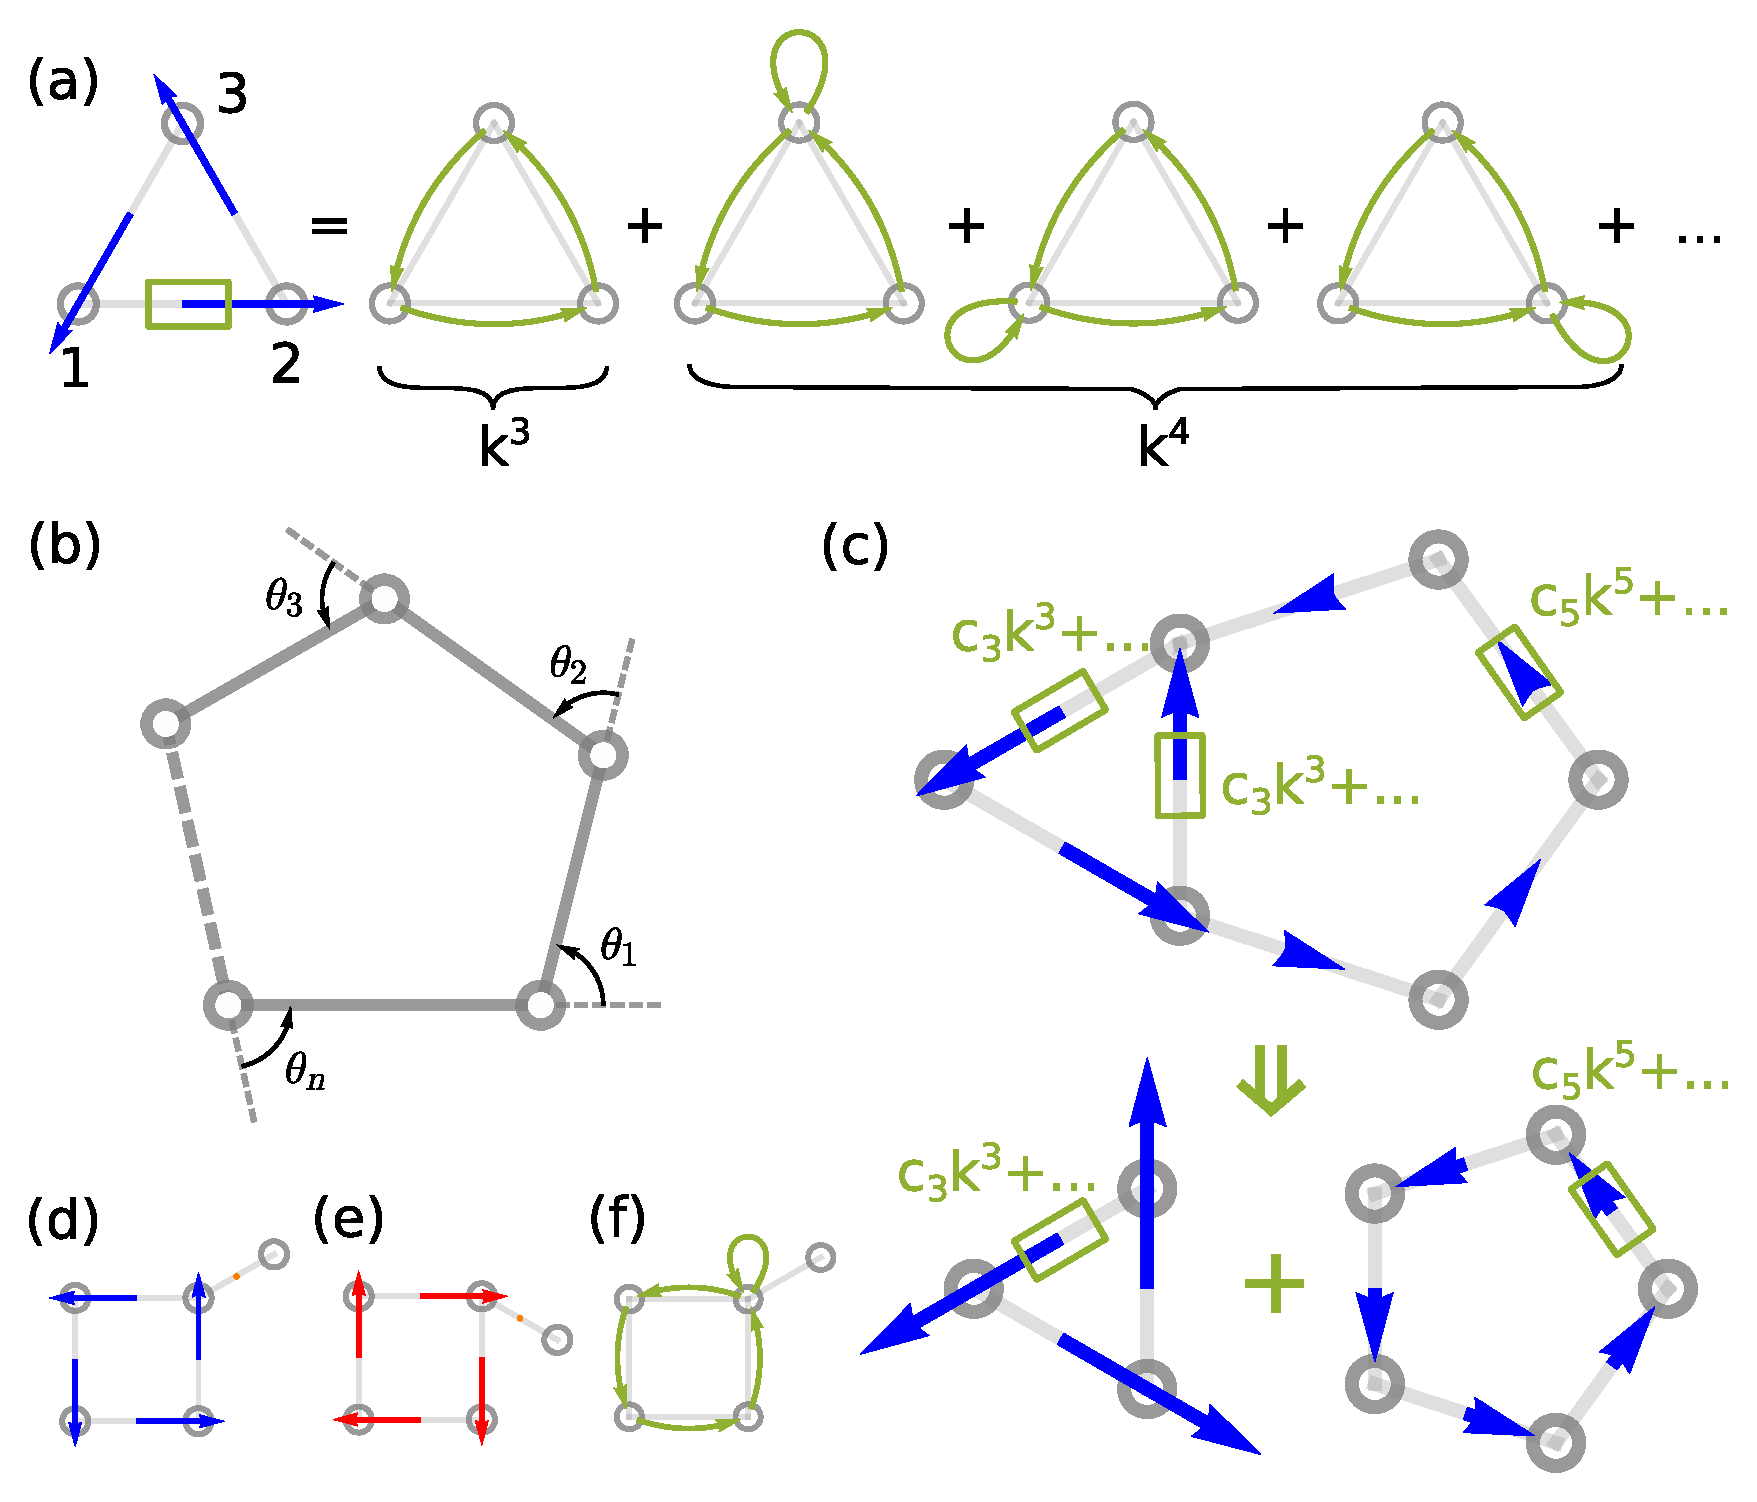
\includegraphics[width=0.45\textwidth]{4_path_sum.pdf}
    \caption{Illustrations of the path summation method.
    (a) Flux from $1$ to $2$ can be calculated by summing over paths. Each path is a diagrammatic representation of one term in the small-$k$ expansion, and is depicted using green arrows. The magnitude of path with length $n$ is on the order of $k^n$.
    (b) Schematic of a polygon path and its outer angles $\theta_1,\theta_2,\dots,\theta_n$. The flux of this path is simply \eqnname~\eqref{eqn:flux_path_polygon}.
    (c) For flux in complex networks, the leading order term is determined by the shortest cycles. Flux in the triangle part has order $k^3$, and the pre-factor $c_3$ is the same as that in a standalone triangle network. Likewise for the pentagon part. So the flux in a complex network can be viewed as a result of ``stitching" flux in its cyclic components together.
    (d-f) Direction of flux can be controlled by the orientation of the side-chain. This is because the flux of the lowest-order path (square) vanishes, and the first non-vanishing path (f) is affected by the side-chain.
    }
    \label{fig:path_sum}
\end{figure}

In this section we develop a diagrammatic expansion of the energy flux. This expansion provides a simple intuitive method to compute energy fluxes and reveals a relationship between flux and network geometry. The {\it{small}} parameter of our expansion will be the spring constant $k$ of the interparticle interactions. We first expand the above derived expressions for the energy flux in small-$k$ regime and show that it can be expressed as sum over paths traversed along the network (\eqnname~\eqref{eqn:flux_path}). Our perturbation theory assigns a geometry dependent pre-factor for each path, thus allowing us to construct a diagrammatic representation for the rectified energy fluxes (Eq \eqnname~\eqref{eqn:flux_path_polygon}). The central results of this section, Eq.~\ref{eqn:flux_path}, Eq.~\ref{eqn:flux_path_polygon} provide compact expressions that elucidate how geometry, $B$ field and $\tau$ can combine to generate energy flows in networks with arbitrarily complex topologies.
%Our diagrammatic theory identifies the important features of the network and active bath that control the energy flux.

%We then also show two situations where polygon paths vanish and higher-order paths (with loops) become dominant.
%Although these quantitative conclusions are based on small-$k$ expansion, they also qualitatively agree with many numerical examples at larger $k$'s.
%Finally, we discuss how the path analysis reveals a simplified dependence of flux on parameters.

\subsection{Path summation and its rules}
Starting from the flux formula \eqnname~\eqref{eqn:flux_residue}, one can expand the flux to different orders in the spring constant $k$. Then for each order, one can further expand to different paths.
As a result, the total flux can be written as a sum over the flux of paths (\figurename~\ref{fig:path_sum}a), (Supplemental Material)
\begin{equation} \label{eqn:flux_path}
    \frac{\expval{J}}{T_a/\tau} = \sum_l J^\text{path}_l = \sum_l \frac{1}{2}(S_l - S_{-l}).
\end{equation}

The path rules are as follows.
For the flux from $i$ to $j$, valid paths are $l=i\rightarrow j\rightarrow l_3\rightarrow l_4\rightarrow \dots \rightarrow l_n\rightarrow i$, where $l_a$ and $l_b$ either has to be bonded or $l_a=l_b$. Paths that contain equal numbers of $i\rightarrow j$ and $j\rightarrow i$ do not contribute (e.g. path $i\rightarrow j\rightarrow i$), because either the path itself vanishes or it cancels with another path. As a result of this, paths appear as cycles.
The term $S_l$ is defined as $S_l \equiv (\frac{k}{k_0})^n \tr R_\alpha (-K_s)_{i l_n} \cdots R_\alpha (-K_s)_{l_3j} R_\alpha (-K_s)_{ji}$,
where $k_0\equiv \sqrt{(k_{g,\tau})^2 + (B/\tau)^2}$ sets the characteristic scale with dimension $k$,
\begin{equation}
\label{eq:alphadefine}
\alpha = \arctan{\frac{B/\tau}{k_{g,\tau}}}
\end{equation}
is a geometric factor, $R_\alpha$ is a CCW rotation by angle $\alpha$, and $(K_s)_{l_b l_a} \equiv \frac{1}{k}\bra{l_b}(K-k_gI)\ket{l_a}$ is the geometric factor of spring force on $l_b$ due to the displacement of $l_a$.
$-l$ means $l$ in the reversed order.
The interval of convergence depends on the geometry of the whole network as well as the parameter $\alpha$. The typical value of the upper bound of $\frac{k}{k0}$ ranges between $0.3$ and $0.6$.

The paths can be represented using diagrams, from which the flux $J^\text{path}_l$ can be calculated easily. For instance, the first diagram in \figurename~\ref{fig:path_sum}a represents the path $1\rightarrow 2\rightarrow 3\rightarrow 1$. To calculate $S_l$, one writes $(-K_s)_{l_bl_a}$ for each arrow $l_a\rightarrow l_b$, $R_\alpha$ for each node $l_a$, then multiply these matrices in the reversed order, and calculate the trace, e.g. $S_{1\rightarrow 2\rightarrow 3\rightarrow 1} = (\frac{k}{k_0})^3 \tr R_\alpha (-K_s)_{13} R_\alpha (-K_s)_{32} R_\alpha (-K_s)_{21}$. To get $S_{-l}$, one takes the result of $S_l$ and replace $\alpha$ by $-\alpha$. Finally, $J^\text{path}_l$ can be calculated from the difference between $S_l$ and $S_{-l}$.

\subsection{An example calculation: Polygonal paths}
Path with length $n$ is on the order $(\frac{k}{k_0})^n$, so that in the small $k$ regime, the main contribution to the flux comes from the lowest-order paths.
The usual lowest-order paths are polygonal cycles with no loops (loops have the form $l_a\rightarrow l_a$), in which case, the formula for $J^\text{path}_l$ \eqnname~\eqref{eqn:flux_path} reduces to a simple form (Supplemental Material)
\begin{equation} \label{eqn:flux_path_polygon}
    J^\text{path}_\text{polygon} = \frac{1}{2} (\frac{k}{k_0})^n (\prod_i \cos(\theta_i - \alpha) - \prod_i \cos(\theta_i + \alpha)),
\end{equation}
where $\alpha$ is defined in Eq.~\ref{eq:alphadefine}, $n$ is the number of nodes and $\theta_i$'s are outer angles (\figurename~\ref{fig:path_sum}b).

For polygon networks, this formula gives a direct relationship between the lowest-order flux and the network geometry, and all parameters are condensed into a geometric angle $\alpha$. As an example, flux in an arbitrary triangle is $J \propto k^3 \sin\theta_1\sin\theta_2\sin\theta_3 + \mathcal{O}(k^4)$, whose $k^3$ term is always positive or CCW.
For complex networks, this formula tells that its lowest-order flux can be viewed as a result of combining the flux of its constituent polygons together, as illustrated in \figurename~\ref{fig:path_sum}c. This is because the flux of a polygonal path \eqnname~\eqref{eqn:flux_path_polygon} is not affected by any side chains on the nodes, and $J^\text{path}_\text{polygon}$ for a polygon in a complex network is the same as $J^\text{path}_\text{polygon}$ for the polygon when standalone.
%Unlike in polygonal paths, paths with loops are affected by side-chains.
%One situation is when the polygon path itself vanishes. In \figurename~\ref{fig:path_sum}d,e, the flux of lowest order path, square, is zero, so the main contribution comes from the path with length $5$, as shown in \figurename~\ref{fig:path_sum}f. Through the loop in this path, the orientation of the side-chain controls the flux direction in the main square, without changing the geometry of the main cycle (as in \figurename~\ref{fig:model_and_result}c-e).

%By changing the network geometry $\theta$, the decay length varies non-monotonically, and has a cusp at $\theta=\alpha$ (\figurename~\ref{fig:path_decay}c).
%This decay and its relationship with $\theta$ can be explained by considering the paths.
%While the hexagon path constitutes the lowest-order path at the boundary, it vanishes for $n_l\ge 1$ due to cancellations. The first non-vanishing pair of paths for $n_l=1$ is shown in \figurename~\ref{fig:path_decay}d, in which the loop exploits the asymmetry between the bulk side (has a vertical bond at the blue loop) and the boundary side (has no vertical bonds at the red loop). For every increment of one layer, the length of paths increases by $4$. So the flux at layer $n_l$ is on the order of $k^{4n_l+3}$, which exhibits an exponential decay $e^{-(n_l-1)/d_l}$.
%Through the calculation of these paths, one gets the decay length $d_l = -1/\log[4(k/k_0)^4(\sin(\theta+\alpha)\sin(\theta-\alpha))^2]$. From this result, we see that the cusp at $\theta=\alpha$ in \figurename~\ref{fig:path_decay}c is due to the term $\sin(\theta-\alpha)$. In fact, at the special point $\theta=\alpha$, paths like \figurename~\ref{fig:path_decay}d vanish, and one needs to consider even high-order paths.

Starting from the  diagrammatic expansion, the presence of localized energy fluxes in such networks can be understood. Consider for instance the paths contributing to flux along a link in a honeycomb-like network (\figurename~\ref{fig:path_decay}). Away from the boundary, the dominant lower order path contributions to the energy flux cancel each other. The size of the leading order path that contributes to the energy flux along a link increases as a function of the distance of the link from boundary. Such a scaling results in an exponential localization of the energy flux at the boundary of the lattice (\figurename~\ref{fig:path_decay}b).
\begin{figure}[ht]
	\centering
	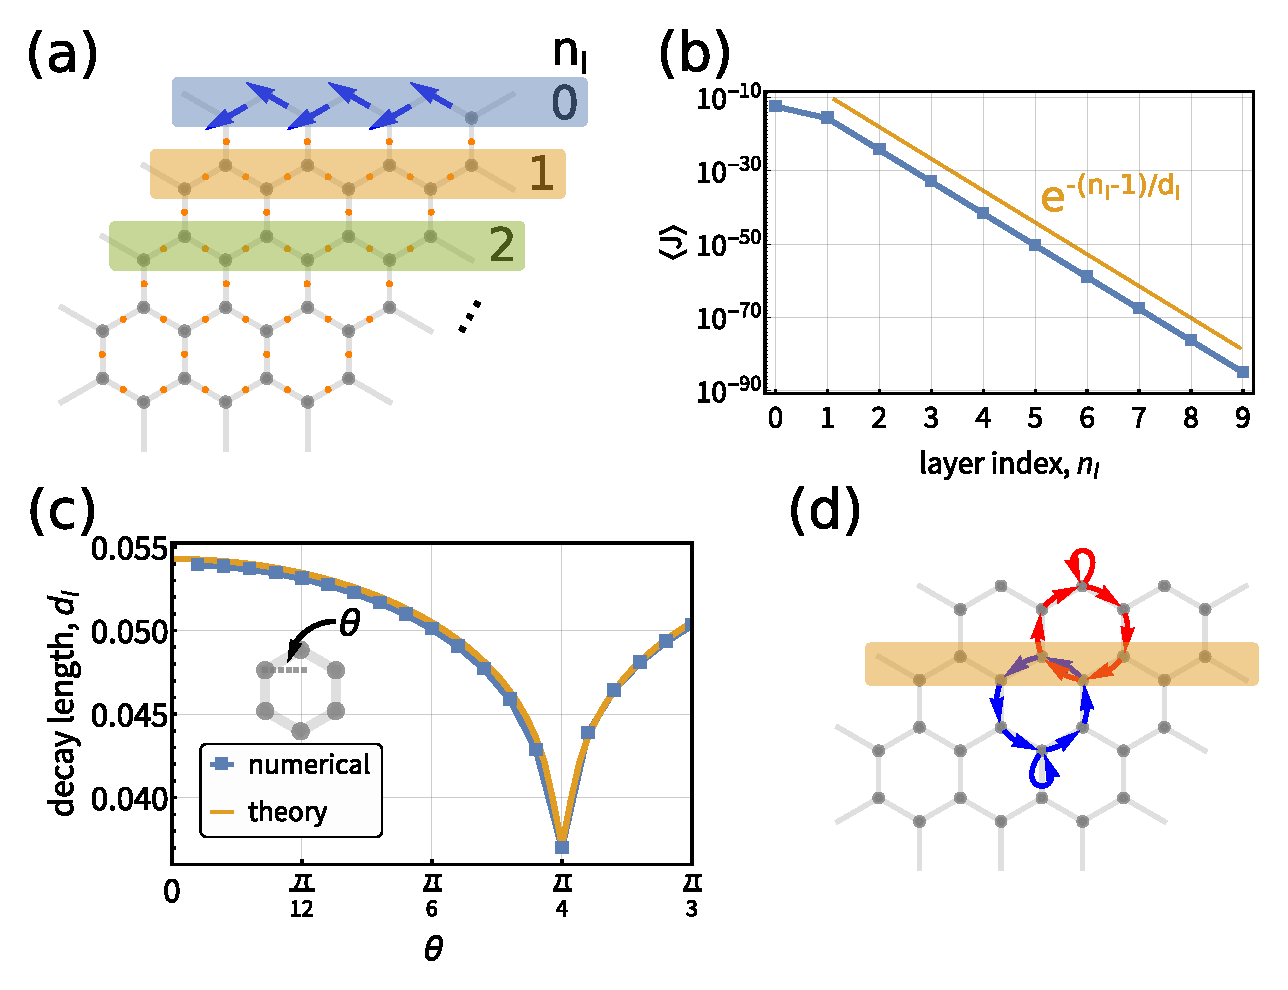
\includegraphics[width=0.45\textwidth]{5_path_decay.pdf}
    \caption{Decay of fluxes away from the boundary of honeycomb networks, and explanation using the path picture.
    (a) Schematic of a honeycomb network which is periodic in the $x$ direction. Layers from the boundary are indexed as $n_l$.
    (b) Semi-log plot of flux $\expval{J}$ at layer $n_l$. The flux starting from layer $n_l=1$ shows exponential decay, with decay length $d_l$. Parameters: $\theta = \pi/6, k/k_0 = 0.01, \alpha = \pi/4$.
    (c) Decay length $d_l$ changes with the network angle $\theta$ non-monotonically, and the curve has a cusp at $\theta = \alpha = \pi/4$. At small $k/k_0$, perturbation theory results agree with numerical calculations.
    (d) The first non-vanishing path pair for $n_l=1$ has length $7$. The two paths do not cancel, because the loop in the bulk and at the boundary have different values.
    }
    \label{fig:path_decay}
\end{figure}

More generally, using these decompositions, it is easy to program energy flux patterns in networks of arbitrary complexity. Our diagrammatic expansion hence allows us to go beyond the need for de novo calculations suggested by our previous expressions.


\section{Coupling the energy flux to fluid pumping} \label{sec:swimmer}

\begin{figure}[ht]
	\centering
	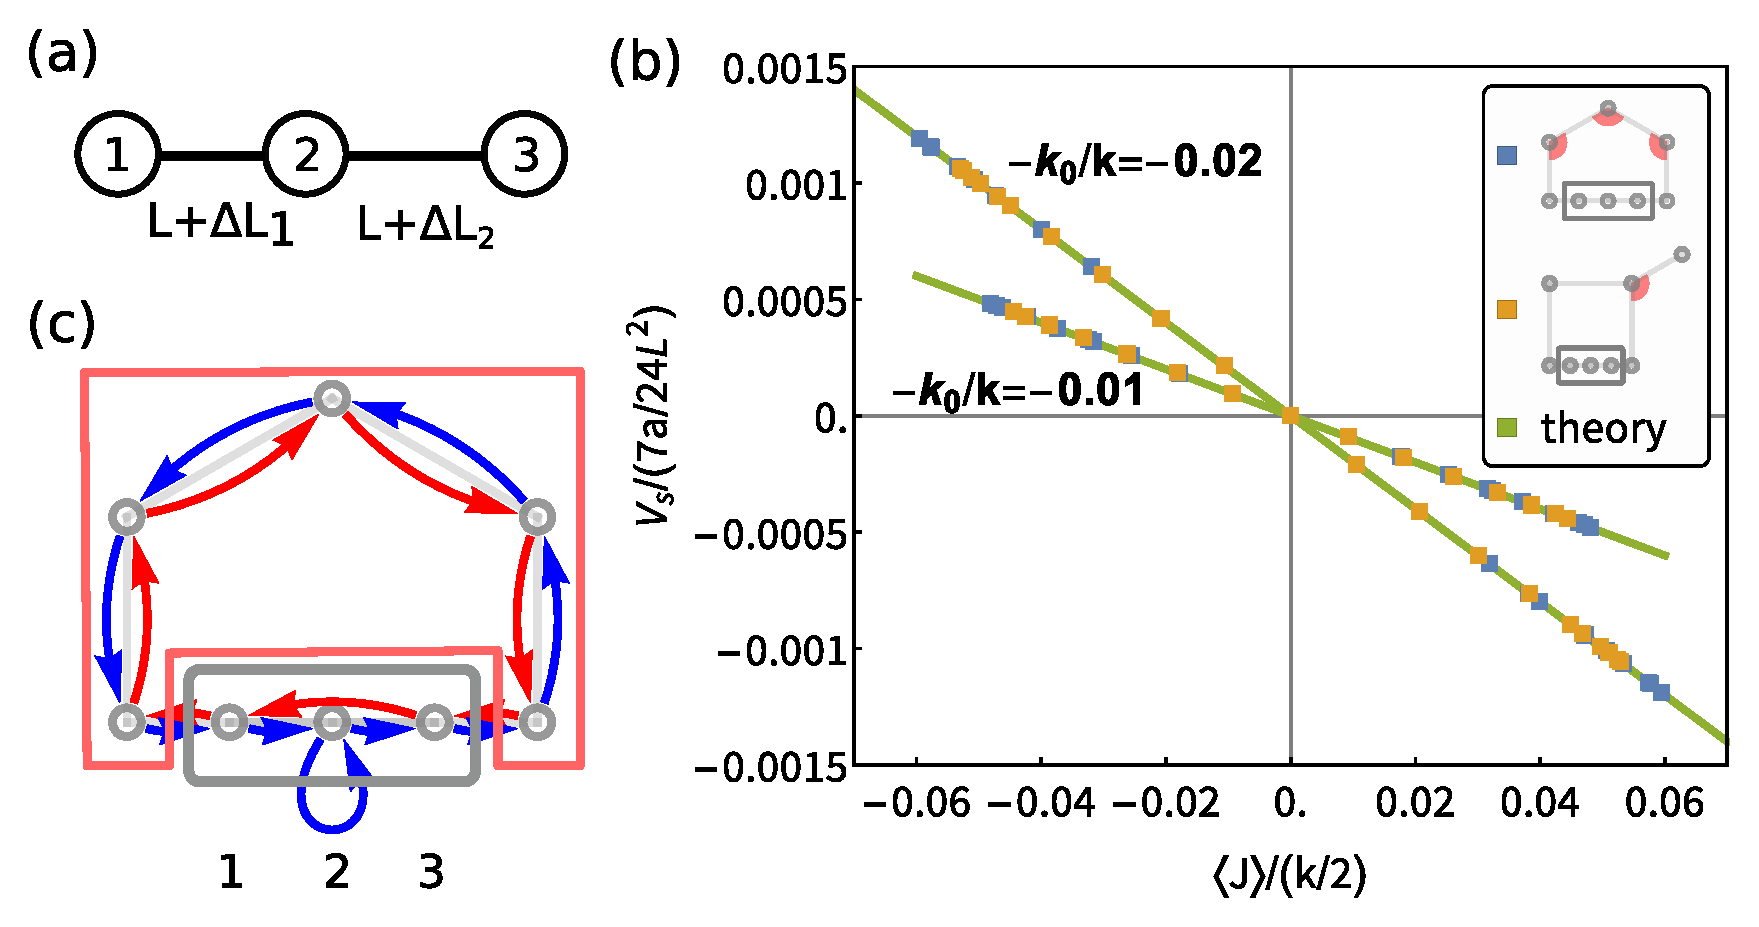
\includegraphics[width=0.45\textwidth]{7_swimmer.pdf}
    \caption{Active network dynamics as a swimming protocol.
    (a) Conventional heat conduction in a chain with temperature differences at two ends. The temperature difference drives a heat flow through a passive material (boxed in gray).
    (b) Similar to (a), the active gyroscopic network can also drive a heat flow through a passive segment. In the simulation setup, the separation between active particles (boxed in red) is large compared with the length-scale of their displacements, and their parameters are: $m,k_g,\gamma=0.1, k=10$, others are $1$. Passive particles (boxed in gray) are restrained to 1D, and their $\gamma,T_a,k_g$ are set to $0$.
    (c) Three-sphere swimmer model from \cite{Golestanian2008AnalyticResults}. In order to swim, the swimmer vary the lengths of its two legs according to some protocol.
    (d) Swimmer's speed $V_s$ is directly proportional to the energy flux $\expval{J}$ in the active network. The proportionality constant is $-k_0/k$, which is independent of the network geometry. The series of dots for each $-k_0/k$ are obtained by varying the labelled angles (by red disk sectors) in pentagon networks or square+tail networks.
    (e) One example of $J_{31}^s$ path (red) and $J_{12}^s$ path (blue). Ballistic particles are boxed in gray, and the active ones are boxed in red.
    }
    \label{fig:swimmer}
\end{figure}

% The energy flux has been our main focus so far. In this section, we show that this energy flux can be used to rectify motion.
% In the first step, we couple the active gyroscopic network to a passive material, and show that energy flux can be driven through the passive elastic object
% Next, noting that the presence of the energy flux requires non-reciprocal motion, we allow the passive elastic object to interact with a highly viscous fluid. We show that the non-reciprocal motion of the constituent particles of the passive elastic object in the viscous fluid can provide a mechanism for propulsion \cite{Golestanian2008AnalyticResults}. Indeed, using the above derived diagrammatic theory, we show that the swim speed of our model system in a viscous fluid is in fact proportional to the energy flux rate. In this manner, designed rectified energy flows can in turn be used to rectify motion and exert forces.

%Since the energy flux indicates some nonreciprocal motion, we then use this motion as a swimming protocol to make a three-sphere swimmer swim.
%After this, we examine the scenario of immersing the passive segment into a fluid and argue that it is possible to pump the fluid.

The rectification of energy has been our main focus so far. In this section, we exploit the energy flux to rectify motion in viscous fluids.
In particular, we discuss the scenario of immersing a segment of the chiral active network into a fluid and illustrate the possibility to pump the fluid.
To make its dynamics cleaner, the segment is set to be passive, or in other words, it does not experience Lorentz force or active bath.
A few preparatory steps are needed before immersion.
First we demonstrate that the passive segment, when coupled to an active network, supports energy flux.
Next we show that the motion of this segment can be used as a swimming protocol, and make a low Reynolds number ($Re$) swimmer swim. Using the diagrammatic theory introduced in \secname~\ref{sec:path}, we will derive that the swimming speed is proportional to the energy flux.
With these preparations, we then discuss the possibility that, the passive segment when immersed in a fluid can act as a stalled swimmer and pump the fluid.

\subsection{Energy flux in a passive segment coupled to an active network}
In the conventional heat conduction, if a passive harmonic chain is placed between two thermal baths with different temperatures, it supports a nonzero averaged energy flux or heat flux (\figurename~\ref{fig:swimmer}a).
Analogously, we can study whether an energy flux can also be generated in the same passive material, but replacing the temperature bias with our chiral active network (\figurename~\ref{fig:swimmer}b).
Numerical calculation (\figurename~\ref{fig:swimmer}b) and simulations (Supplemental Video and Supplemental Material) show that the passive segment does support energy fluxes.
From the Supplemental Video, the flux through the passive segment is in general stochastic. Although the direction of flux is from left to right on average, the instantaneous flux can also transport from right to left. During the period when $J$ is large, $J$ exhibits successive peaks, indicating a large energy flow from left to right. The spacing between the peaks matches the sound speed of the passive chain.


\subsection{Nonreciprocal motion as a swimming protocol}
The energy fluxes through the passive segment, especially the successive flux peaks observed in the above simulation, seem to suggest a stochastic version of wave-like motions. The wave-like motions, in the context of low $Re$ swimmers, is one type of swimming strategies \cite{Taylor1951AnalysisSwimming,Golestanian2008AnalyticResults}. Thus the motions of the passive segment could potentially be exploited as a swimming strategy.

The swimmer model we choose is a linear three-sphere swimmer \cite{Golestanian2008AnalyticResults}, because it is a model with minimal components, and it can readily adopt the motion of our passive segment. The swimmer as \figurename~\ref{fig:swimmer}e is immersed in a low $Re$ fluid. When the swimmer changes the lengths of its two legs according to some protocol, which is described by a constant part $L$ plus a varying part $\Delta L_i$ for $i=1,2$, the time-averaged swimming speed is (\eqnname~(12) in \cite{Golestanian2008AnalyticResults})
\begin{equation} \label{eqn:swimmer_speed}
    V_s = \frac{7a}{24L^2} \expval{\Delta L_1 \Delta \Dot{L_2} - \Delta \Dot{L_1} \Delta{L_2}},
\end{equation}
where $a$ is the radius of the bead. Assumptions for this equation are $a/L \ll 1, \Delta L_i/L \ll 1$, and total external force on the swimmer is zero.

We set the swimming protocol to be the motions of the three passive particles (\figurename~\ref{fig:swimmer}b, except that here we allow $k_g$ of passive particles to be nonzero),
compute $V_s$ of the swimmer and compare it to the energy flux $\expval{J}$ through the passive segment.
The $V_s-\expval{J}$ plot in \figurename~\ref{fig:swimmer}d shows that, the swimmer using our protocol can swim, and the speed $V_s$ is proportional to $\expval{J}$. Moreover, this proportionality constant does not depend on the network geometry.
In fact, this constant can be calculated using a modified path analysis (Supplementary Material),
\begin{equation} \label{eqn:swimmer_propto}
    \frac{V_s}{7a/24L^2} = -\frac{k_0}{k} \frac{\expval{J}}{k/2},
\end{equation}
where $k_0 = k_g + m/\tau^2$ ($B,\gamma=0$ for the passive part).
This result \eqnname~\eqref{eqn:swimmer_propto} holds beyond small-$k$ regime because all orders of paths are considered (\figurename~\ref{fig:swimmer}e, and Supplementary Material).
\figurename~\ref{fig:swimmer}d and \eqnname~\eqref{eqn:swimmer_propto} together establish that one can dictate swimmer's speed from the energy flux of active networks.
Similar proportionality between $V_s$ and $J$ can be expected for other types of three-sphere swimmers, such as one where one sphere is much larger than the other two \cite{Golestanian2008ThreesphereLowReynoldsnumber}. This is because $V_s$ is proportional to the area enclosed in the $\Delta L_i$ space \cite{Golestanian2009StochasticLow}, and this area is proportional to $J$ (Supplemental Material){\bf this seems to be an important statement but currently the writing is not good}.

\subsection{Coupling energy flux to fluid pumping}
Now we consider the scenario where the passive segment is immersed in a fluid. Since the segment is tethered by $k_g$ and is connected to the tethered active part, it cannot swim indefinitely. However, a tethered swimmer is able to pump the fluid \cite{Leoni2009BasicSwimmer}. To see whether the passive segment can also pump the fluid as the swimmer, we need to discuss how the tethering force and the added fluid affects the dynamics of the segment.

In the presence of tethering forces, \eqnname~\eqref{eqn:swimmer_speed} for $V_s$ needs to be modified.
Ref. \cite{Golestanian2008AnalyticResults} discussed swimmer with a constant external force $F$, and its \eqnname~(39) says the modified swimming speed $V_s(F) = V_s + F/(6\pi\eta_f a)$, where $\eta_f$ is fluid's dynamic viscosity.
Since this result is obtained under linearized hydrodynamics, it also applies to our stochastic case granted that we replace $F$ by its averaged value $\expval{F}$.
This tells us that we can first consider the untethered case, then go to the tethered case using the above formula.

In the presence of an added fluid, we would like that the original dynamics is not altered too much, otherwise both the energy flux and the correlation in \eqnname~\eqref{eqn:swimmer_speed} would be distorted, and one cannot utilize the $V_s \propto -\expval{J}$ result.
So we need a regime where the fluid, in spite of having a low $Re$, is perturbative.
To make the fluid perturbative, we need the dissipation rate due to the viscous force to be much smaller than the energy flux through the segment. This can be expressed as $\eta_f a v^2 \ll J$, where $v$ is the velocity of the bead, $J$ is the energy flux in the absence of the fluid.
To satisfy low $Re$ condition, one needs $Re = \frac{\rho_f a v}{\eta_f} \ll 1$, where $\rho_f$ is fluid's density.
Writing these two conditions together, one gets $J \gg \eta_f a v^2 \gg \rho_f a^2 v^3$.
This condition ignored hydrodynamic interactions between the beads, because it is a higher-order perturbation with the order of $a/L$.
As a numerical example, this condition can be satisfied by setting $k=5\times 10^{-5} kg/s^2, k_g=1\times 10^{-6} kg/s^2$ for springs (value of optical trap), $a=10^{-6}m$ for all beads (size used in \cite{Leoni2009BasicSwimmer}), $T_a=10^{-18} J, \tau=1s$ for the active bath \cite{Wu2000ParticleDiffusion}, $\rho_f=10^3kg/m^3, \eta_f=10^{-3}kg/(m\cdot s)$ for liquid (water), and $B=10^{-5} kg/s$ for the $B$-field.
Then from numerical calculations, $v=3.8\times 10^{-6}m/s$, and the three scales are $J=5\times 10^{-19}J/s, \eta_f av^2=1.4\times 10^{-22}J/s, a^2v^3\rho_f=5.4\times 10^{-29}J/s$.
The only suspicious parameter is $B$, which seems to be too strong in order to make $J$ sizable. To make practical use of this model, one should consider Lorentz-like force substitutes, such as gyroscopes.

These discussions together suggest that, if the passive part is immersed in a perturbative fluid, it can generate fluid flows.
Assuming the relaxation timescale of the active network is much faster than the timescale of swimming due to the small $V_s(F)$, one can expect the following process. Initially the passive part experiences $\expval{F}=0$, so it swims with speed $V_s$; as the part drifts, $\expval{F}$ increases and acts in the direction of $-V_s$; when $\expval{F} \approx -6\pi\eta_f a V_s$, the swimmer is stalled. The stalled swimmer pumps fluid in direction $-V_s \propto \expval{J}$.


\section{Conclusion} \label{sec:conclusion}

We have established that, our active gyroscopic network can rectify energy and control its rectification through network geometries.
At last, we discuss possibilities to extend this model and provide outlooks.

In our theoretical treatment, the parameters are assumed uniform for all particles and bonds, which is not necessary. We only need $\tau,T_a$ to be uniform, and other parameters $m, k_g, k, B, \gamma$. can be nonuniform.
If we add an additional white noise to the equation of motion \eqnname~\eqref{eqn:GLE_single}, the energy flux is not affected. As a comparison, in models that use OUP for directed particle transport, the additional white noise would usually suppress the rectification \cite{Bartussek1996PreciseNumerics}.

From Fourier mode analysis (\secname~\ref{sec:fourier}), the ingredients for nonzero energy fluxes are nonreciprocal response and weighted excitation.
The nonreciprocal response is introduced by Lorentz-like forces, and it makes theory tractable, since this force does not do work on the particles and is linear. The disadvantage is that its experimental realization is not easy.
Inspired by these two ingredients, one can try other ways to achieve rectifications.
One way is to replace the active particle with Lorentz force by active rotors. In this case the equation for energy flux \eqnname~\eqref{eqn:flux_integral} would contain extra terms, and since rotors themselves are active, the active bath is not needed.
Another possible way is to introduce nonlinearity, as nonlinearity can make nonreciprocal metamaterials  (cite nonreciprocal). This has been exploited to make thermal diodes. One could imagine a setup that replaces the springs with these nonreciprocal materials, and add active bath but not Lorentz force to the connecting sites.

% outlook
% active matter + network structure. cite Woodhouse's work, search for others.


\section*{Acknowledgements}
We thank many people.


\bibliography{reference}

\end{document}
